\begin{figure}[H]
	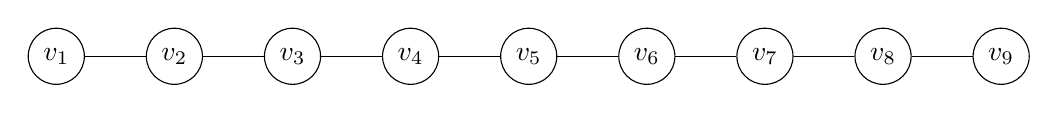
\begin{tikzpicture}[node distance={15mm}, main/.style = {draw, circle}]
		\node[main] (1) {$v_1$};
		\node[main] (2) [right of=1] {$v_2$};
		\node[main] (3) [right of=2] {$v_3$};
		\node[main] (4) [right of=3] {$v_4$};
		\node[main] (5) [right of=4] {$v_5$};
		\node[main] (6) [right of=5] {$v_6$};
		\node[main] (7) [right of=6] {$v_7$};
		\node[main] (8) [right of=7] {$v_8$};
		\node[main] (9) [right of=8] {$v_9$};
		\draw (1) -- (2);
		\draw (2) -- (3);
		\draw (3) -- (4);
		\draw (4) -- (5);
		\draw (5) -- (6);
		\draw (6) -- (7);
		\draw (7) -- (8);
		\draw (8) -- (9);
	\end{tikzpicture}
	\centering
	\caption{Structure $\mathfrak{G}_1$, consisting of a line of length $8$.}
\end{figure}